%caracteristicas
\section{Características}

\subsection{Alta velocidad de decodificación}
La alta velocidad de decodificación permite minimizar el tiempo de lectura y, también utilizarlos en dispositivos con recursos de computación limitados.\cite{2012_Encinas}

\subsection{Bajo coste del decodificador}
Los códigos bidimensionales QR solo necesitan una cámara de baja resolución para capturar el código y software para procesarla. Es posible, usar télefonos moviles o una webcam. Para el decodificado del código, existen numerosas implementaciones en software de uso libre o código abierto y librerías.\cite{2012_Encinas}

\begin{figure} 
\centering
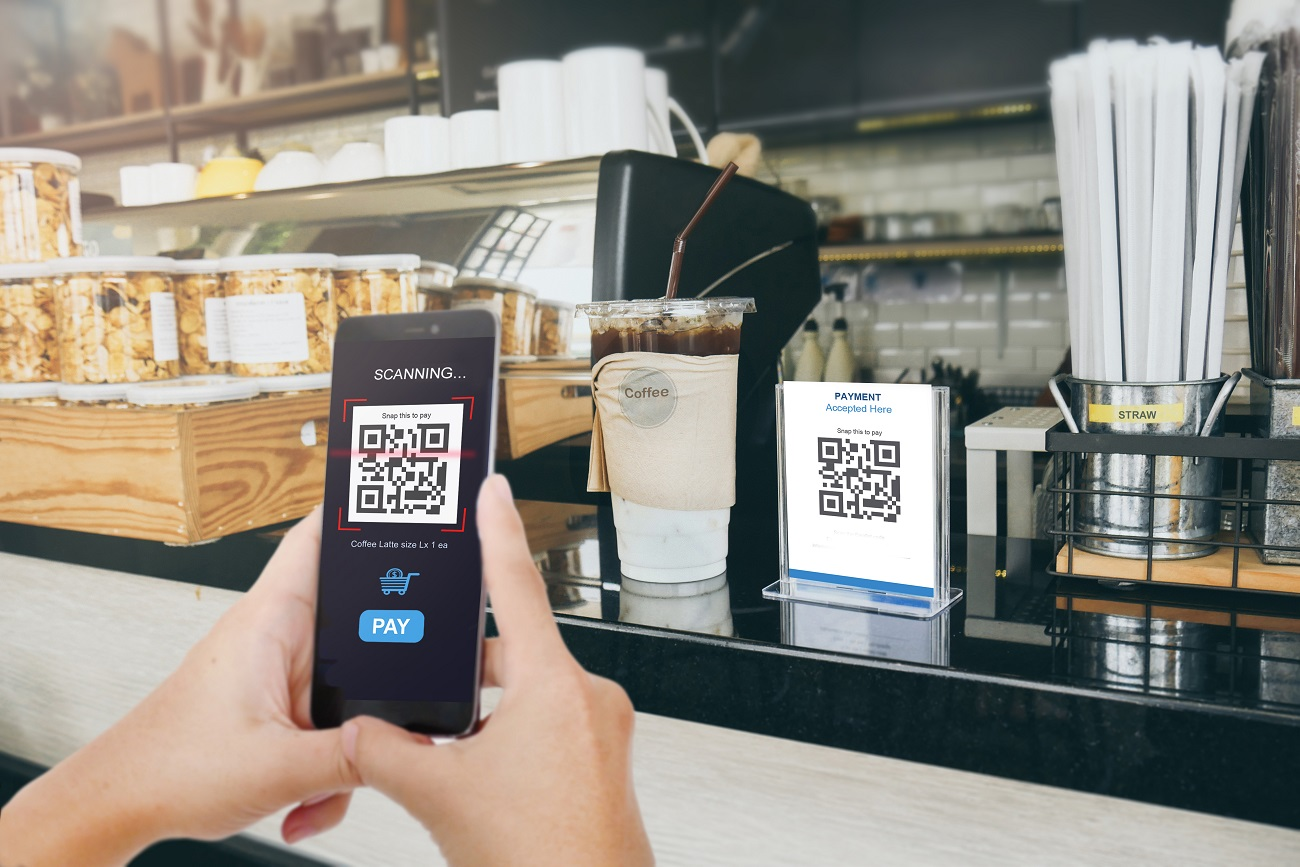
\includegraphics[width=0.4\textwidth]{escanear-codigo-qr.jpg}
\caption{Lectura de los códigos QR, mediante una aplicación.}
\label{fig:costedecodificador}
\end{figure} 

\subsection{Facilidad de lectura}
Un código QR puede ser leído desde cualquier dirección en 360 grados. Esto es posible debido a los patrones de detección de posición en las tres esquinas del símbolo, hacen que el código QR se pueda identificar y leer de forma rápida.\cite{2014_Chang}
Los patrones permiten reorientarlo automáticamente una vez que son capturados por la cámara, eliminando cualquier interferencia de fondo, lo que garantiza una lectura estable de alta velocidad.\cite{2012_Encinas,2012_DENSO}


\subsection{Gran capacidad de codificación de datos}
Los códigos de barras tradicionales solo almacenan hasta 20 dígitos. En cambio, la característica más importante del código QR es la codificación de datos, puede proporcionar hasta 200 veces más información que los códigos de barras unidimensionales. El código QR puede codificar hasta poco más de 7,000 caracteres o 300 caracteres alfanuméricos.\cite{2014_Chang,2012_DENSO} Dependiendo del tipo de dato a codificar la capacidad del código QR varia, siendo superior a la de otros códigos bidimensionales.   Por ejemplo, si los datos son numéricos, el máximo es de 7,089 caracteres; si son alfanuméricos, el máximo es de 4,296 caracteres; en cambio, si son binarios, el máximo es de 2,953 bytes.\cite{2012_Encinas}
%highcapacitydatastorage
\begin{figure} 
\centering
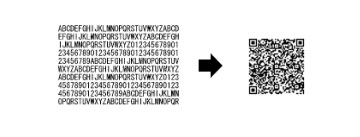
\includegraphics[width=0.7\textwidth]{highcapacitydatastorage.jpg}
\caption{Un código QR de este tamaño puede contener 300 caracteres alfanuméricos.}
\label{fig:datastorage}
\end{figure} 

\subsection{Gran resistencia frente a errores y daños}
El contenido en un código QR es posible recuperarla, aunque parte del mismo tenga errores, este dañada o manchada.\cite{2012_Encinas}
Para recuperar la información, el código QR tiene la capacidad de realizar corrección de errores. La restauración de datos depende de la proporción del daño que tiene el símbolo.\cite{2014_Chang}
%ErrorCorrectionCode.jpg
\begin{figure} 
\centering
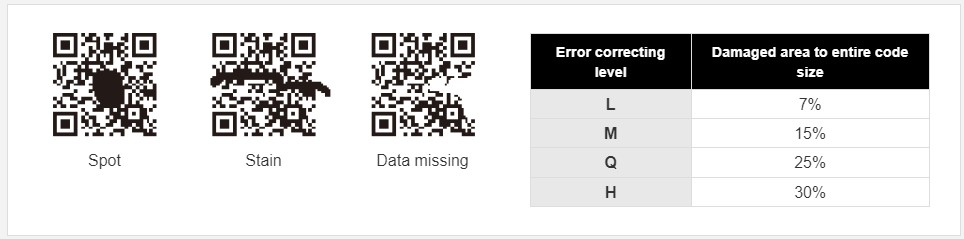
\includegraphics[width=0.9\textwidth]{ErrorCorrectionCode.jpg}
\caption{El código Reed-Solomon se aplica para restaurar los datos cuando una parte del código QR falta o está dañada. La tasa de restauración varía en 4 niveles diferentes de corrección de errores.}
\label{fig:ErrorCorrectionCode}
\end{figure} 

De acuerdo con el nivel de corrección de errores elegido, se puede decodificar hasta un máximo del 30\% de los datos si están sucios o dañados. Un símbolo de código QR se puede leer incluso si su imagen está curvada o distorsionada. \cite{2012_DENSO}
El código Reed-Solomon se desarrolló originalmente como una medida contra el ruido de comunicación para sondas planetarias y para satélites artificiales. Siendo uno de los métodos matemático de corrección de errores usados en los discos compactos de música, es capaz de realizar la corrección a nivel de bytes, y es adecuado para códigos de errores de ráfaga concentrados.\cite{2004_Ohmsha,2008_Conf}
En cambio, si uno o más de los patrones de detección de posición en las tres esquinas del símbolo es borrado o eliminado, no sera capaz de reorientarlo automáticamente, por ende, incapaz de decodificarlo.
\begin{figure} 
\centering
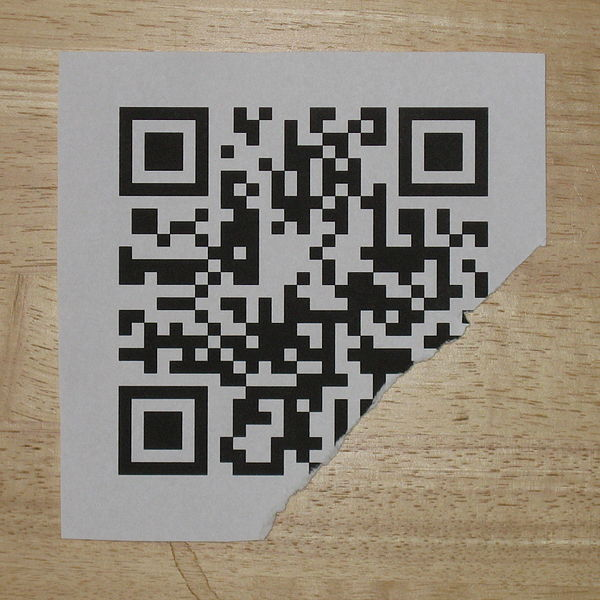
\includegraphics[width=0.3\textwidth]{QR_Code_Damaged.jpg}
\caption{Código QR dañado pero es capaz de decodificarse.}
\label{fig:ErrorCorrectionCode1}
\end{figure} 

\subsection{Posibilidad de personalización}
El símbolo de código QR tiene una estructura bidimensional, se puede usar un código micro QR para un tamaño de impresión más pequeño.
Dado que tiene una gran resistencia frente a errores y daños, los códigos QR se pueden personalizar añadiendoles color, superponiendo algún elemento propio de la imagen de alguna empresa o modificando alguna parte del código.\cite{2014_Chang,2012_Encinas}
\begin{figure} 
\centering
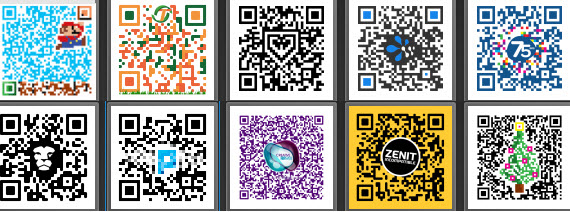
\includegraphics[width=0.7\textwidth]{codigos-qr-creativos-logos.jpg}
\caption{Códigos QR personalizados}
\label{fig:qrpersonalizados}
\end{figure} 


\subsection{Adaptación al tamaño de los datos}
Un código QR puede contener la misma cantidad de datos que un código de barras unidimensional en solo una décima parte del espacio.\cite{2012_DENSO}
Dependiendo de la cantidad de datos a codificar en el símbolo de código QR, el estándar permite utilizar hasta 40 versiones. Cada versión tiene mayor capacidad de codificación que la anterior, a mayor cantidad de datos a codificar; mayor será la versión. Las versiones solo quedan definidas por el número de módulos que se utilizan para su representación. El elemento más pequeño (celda blanca o negra) del código QR se llama ``un módulo''. \cite{2012_Encinas}
\begin{figure} 
\centering
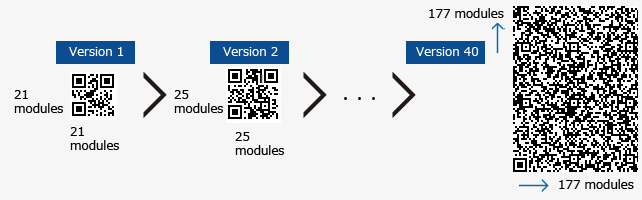
\includegraphics[width=0.7\textwidth]{versionVarietyImage.png}
\caption{Versiones del código QR}
\label{fig:Versiones}
\end{figure} 
Otra característica del código QR es su característica de anexión estructurada. Permitiendo imprimir su estructura en un espacio más reducido. En otras palabras, un símbolo de código QR pueden contener hasta 16 símbolos más pequeños separados, cada uno de los cuales contiene información única. También es posible dividir un solo símbolo de código QR entre cuatro diferentes códigos QR.\cite{2014_Chang}
%qrdivide4.png
\begin{figure} 
\centering
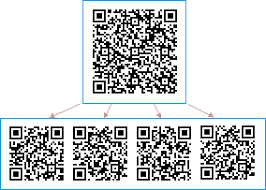
\includegraphics[width=0.5\textwidth]{qrdivide4.png}
\caption{El código QR único se puede dividir en cuatro códigos diferentes.}
\label{fig:qrdivide4}
\end{figure} 

